\chapter{Filtrering af signal}
I dette kapitel designes et båndstopfilter med endelig impulsrespons (altså et FIR-filter), der har til formål at eliminere den midterste frekvens ved $\omega_2 = \frac{\pi}{2}$ mest muligt og samtidig reducere de øvrige frekvenser ved $\omega_1 = \frac{\pi}{3}$ og $\omega_3 = \frac{3\pi}{4}$ mindst muligt. I kapitlet beskrives først specifikationerne og design af filteret, hvorefter... Til sidst perspektiveres der til et IIR-filter som alternativ til FIR-filteret.
\section{Specifikationer} \label{ch4_specs}
FIR-filteret vælges til at være af type 1, altså er filterordenen $M$ lige og impulsresponsen $h[n]$ er symmetrisk, så $h[n] = h[M - n]$. Filteret har 2 knækfrekvenser $\omega_{c_1}$ og $\omega_{c_2}$ i rad/s, som vælges til at ligge symmetrisk omkring $\omega_2$, der skal elimineres ved hjælp af filteret:
\begin{align*}
\omega_{c_1} &= \omega_2 - \delta, \\
\omega_{c_2} &= \omega_2 + \delta,
\end{align*}

hvor $\delta$ vælges til at være $\frac{\pi}{15}$. Filteret designes dermed som et båndstopfilter med ovenstående knækfrekvenser. Den ideelle amplituderespons $H_d(\text{e}^{j\omega})$ er skitseret på figur \ref{fig:ideel_amp_respons} ud fra de opstillede specifikationer.   
\begin{figure}[H]
    \centering
    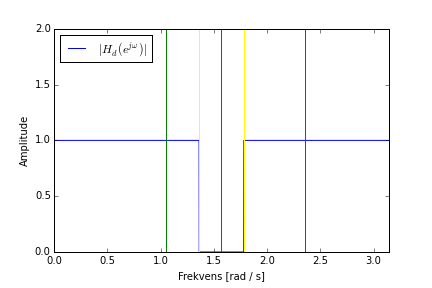
\includegraphics[width = 0.6\textwidth]{figures/ideel_amp_respons.PNG}
    \caption{Den ideelle amplituderespons for filteret. De to grønne streger markerer $\omega_1$ og $\omega_3$, som skal beholdes, og de to gule streger markerer $\omega_{c_1}$ og $\omega_{c_2}$, som ligger symmetrisk omkring den røde streg, der markerer $\omega_2$, som skal elimineres.}
    \label{fig:ideel_amp_respons}
\end{figure}


\section{Vurdering}
\section{Vurdering}
På bagrung af graferne i sektion \ref{resultater} kan det konkluderes at det designede FIR filter af orden ?? formår at filtrere frekvensen $\omega_2=\frac{\pi}{2}$ fra det samplede signal $s[n]$, som ønsket.\\
Figur \ref{amplitude respons} illustrerer at de opstillede specifikationer til en vis grad overholdes ved en orden på hhv. 30 og 100 og anvendelse af det reksangulare vindue. Dog ses det tydeligt at transitionsbåndet bliver smallere jo højere orden der anvendes. De ripples der forekommer i passbåndet formindske ligeså, som ordnen øges, dog forsvinder de ikke som resultat at at det er det rektangulere vindue der anvendes. Som nævnt kan dette optimeres ved at ændre vinduet, hvilket undersøges nærmere i næste afsnit. \\
Figur \ref{filt signal i frekvens} illustrere yderligere hvorledes den ønskede frekvens er fjernet, uden at fjerne de omkring liggende frekvenser. Dog ses som resultat af de forekommende  rippels i passbåndet at amplituderesponsen på de tilbageværende frekvenser forvrænges en smule.    
Ved sammenligning af amplituderesponsen for det designede filter \ref{?} og den ideelle amplituderespons, skitseret på figur \ref{?}, vurderes det altså at det designede filter kan optimeres yderligere. \\
          


\section{Optimering}
